
\lecture{10}{2025-03-20}{intro to CAD and Verilog}{}
\begin{parag}{Previously on FDS}
\begin{itemize}
    \item We implemented $+/-$ arithmetic circuits using logic gates
        \begin{itemize}
            \item Basic building blocks: full adder and subtractor
            \item $N$-bit ripple carry adder in two's complement
        \end{itemize}
    \item Discovered the importante of circuit delay (Examples of critical path delay computation)
    \item Built fast adders: Carry-select adder
    \item Barrel shifters
        \begin{itemize}
            \item Used multiplexers to perform logic arithmetic shift
        \end{itemize}
\end{itemize}
\end{parag}

    \section{Computer Aided Design}
    \begin{parag}{Introduction to CAD tools}
        Logic circuit found in today's complex computing systems cannot be designed manually, Designers of logic circuits heavily rely on the availability of \important{computer-aided design (CAD)} tool:
   \begin{center}
       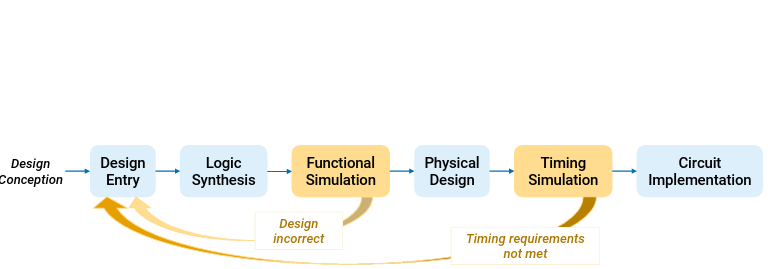
\includegraphics[scale=0.6]{12025-03-20.png}
   \end{center}
    
    \end{parag}
   \begin{parag}{Design Entry}
       Design entry is the starting point in the process of designing a logic circuit. The conception of what the circuit is supposed to do and the formulation of its general organization and structure. It the perfomrd by the designers without the guidance of CAD tools, it requires experience and intuition.
       \begin{subparag}{Approach $1$: Schematic capture}
           The goal here is to draw the logic gates and interconnecting them with writes, schematics tools provide libraries of gates and other circuit components.
           \begin{itemize}
               \item \important{Hierachical design}: Subcircuits previously created can be represented as graphical symbols and included (reused) in the schematic
           \end{itemize}
           
       \end{subparag}
       \begin{subparag}{Approach $2$: Hardware description language}
           An HDL is similar to a typical computer programming language exept that an HDL is used to describe hardware rather than a program to be executedd on a computer\\
           Mainstram HDL languages supported by vendors of digital hardware technology annd officially endorsed as IEEE standards:
           \begin{itemize}
               \item \important{Verilog HDL (cs-173)} and VHDL
           \end{itemize}

       \end{subparag}
       
   \begin{subparag}{HDL vs. Schematic capture}
       HDL's supported by many companies: no need to change the design from one company to another $ \implies$ Easy \important{portability}.\\ 
       Design entry means writing verilog source code, the code is plaint text which make it easy to include in the documentation $ \implies$ \important{Easy sharing and reuse}.\\
       Similar to schematic capture, HDLs support \important{hierachical design}\\
       HDL source can be \important{combined} with schematic capture (e.g., a subcircuit)
   \end{subparag}
   \end{parag}
    \begin{parag}{Functional simulation}
        A circuite described in the form of logic function can be simulated to verify that it will work as expected.\\
        Functional simulators assume the logic functions will be implement with \important{perfect gates (zero-delay model)}\\
       For the sequence of \important{inputs specified by the designers}, the simulator evaluates the circuit outputs and produces the results (e.g., \important{timing waveforms}) to be analyzed by the designers. Most often the result of this is a time diagram.
    \end{parag}
    
    
    \begin{parag}{Physical Design}
        \important{Mapping} a circuit described in the form of logic expression into a realization that uses logic gates or other hardware components available\\
        \important{Placement} Determine the absolute and relative location of the hardware components on physical chip\\
        \important{Routine} Determine the location and shape of the wiring connections that have to be made between the inputs and outputs of the hardware components to connect them appropriately.
    \end{parag}
    
    
   \begin{parag}{Timing simulation}
       Real circuits cannot perform their function with zero delay\\
       \important{llogic propagation delay}: Logic element need time to generate a valid output whenever there are changes in the value of their inputs\\
       \important{Wire propagation delay}
   
   \end{parag}
   
   \begin{parag}{Circuit implementation}
       Having ascertained that the circuit meets all desired requirements, the circuit is ready to be implemented on an actual chip\\
       \textbf{Option ahead}
       \begin{itemize}
           \item Chip fabrication (+ highest performance - extremely expensive)
           \item Chip configuration (+ flexible, + affordable, - lower performance)\\
    If a programmable hardware device is used as a baseline, the desired logic functionality can be implemented by simply reprogramming the device configuration
       \end{itemize}
   
   \end{parag}
   
    \subsection{Verilog}
    \begin{parag}{Bried history of verilog}
        \begin{itemize}
            \item HDLs were introduced in the mid 1980s as languages for describing the behavior of a logic circuit
            \item Verilog was invented by Phil Moorby and Prabhu 
                \begin{itemize}
                    \item A propriety language owned by Gateway design automation
                \end{itemize}
        \end{itemize}
    
    \end{parag}
    
   \begin{parag}{Modeling of digital circuits in verilog}
       A logic circuit is specified in the form of a \important{module}
       \begin{subparag}{Option $1$: Structural modeling}
           Gate-level modeling: Using verilog constructs to describe the structure of the circuit in terms of \important{circuit elements}, such as logic gates\\
           A larger circuit is defined by writing code that instantiates the 
           
       \end{subparag}
   
   \end{parag}
    
   \begin{parag}{Structural Modeling with logic gates}
       In structural modeling, predefined modules that implement basic logic gates are used\\
       Logic gate instantiation statement:
       \begin{center}
           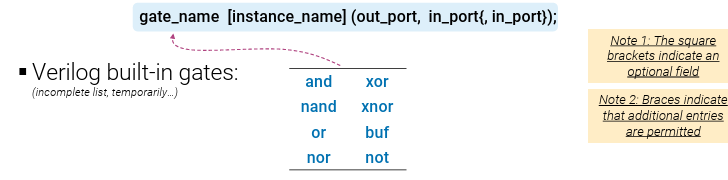
\includegraphics[scale=0.8]{22025-03-20.png}
       \end{center}

       \begin{subparag}{Example}
           Recall logic gate instantion statement:
           \begin{center}
               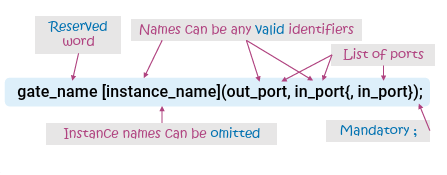
\includegraphics[scale=0.6]{32025-03-20.png}
           \end{center}
           
           
       \end{subparag}
       

   
   \end{parag}
   
      \begin{parag}{Verilog Syntax}
          \begin{subparag}{Names}
             \begin{itemize}
                 \item 
              Must start with a letter
          \item Can contain any letter, number, "\_"
             \end{itemize} 
          \end{subparag}
      
      \end{parag}
     
      \begin{parag}{Modules in verilog}
          Acircuit or subcircuit described with verilog code is a \important{module}. Module has a name, inputs, and outputs, referred to as its \important{prots}
          \begin{center}
              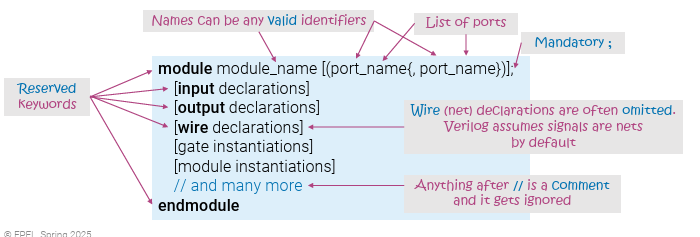
\includegraphics[scale=0.5]{42025-03-20.png}
          \end{center}
          
      
      \end{parag}
      
      
      \begin{parag}{Full adder in verilog}
          \begin{center}
              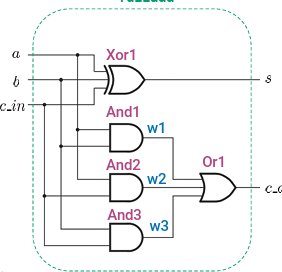
\includegraphics[scale=0.7]{52025-03-20.png}
          \end{center}
         \begin{subparag}{Algorithm}
             \begin{itemize}
                 \item Name your circuit
                     \begin{itemize}
                         \item That will be the name of your verilog module
                     \end{itemize}
                 \item Label all inputs and outputs
                     \begin{itemize}
                         \item Those will be the input and output port names of your verilog module
                             
                     \end{itemize}
                 \item Label all logic gates
                     \begin{itemize}
                         \item Those will be the names of your gates instances
                         \item same gate type can be instanciated multiple times, provided the instance name is unique
                     \end{itemize}
                 \item Label all internal nets
                     \begin{itemize}
                         \item Those will be the names of the wires in your Verilog module
                     \end{itemize}
             \end{itemize}
             
         \end{subparag} 
     \begin{subparag}{Concrete code}
         Here is how the code of the full adder would look like:
         \begin{center}
             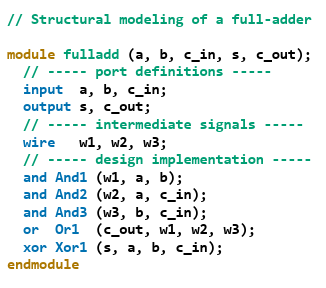
\includegraphics[scale=1]{62025-03-20.png}
         \end{center}
         
         
     \end{subparag} 
      \end{parag}
      \begin{parag}{Subcircuits in Verilog}
          A verilog module can be included as a subcircuit in another module. Modules should be defined in the same source file, in any order (or the verilog compiler must be told where each module is located).
     \textbf{Module instantiation statement } 
     \begin{center}
         \begin{align*}
             \text{module\_name instance\_name(.port\_name ([expression])\{,.port\_name(]expression])\});}
         \end{align*}
         
     \end{center}
    \begin{subparag}{Example}
        For example if we take the full add module created earlier and want to structure a Four-bit ripple Carry Adder, it would gives us:
        \begin{center}
            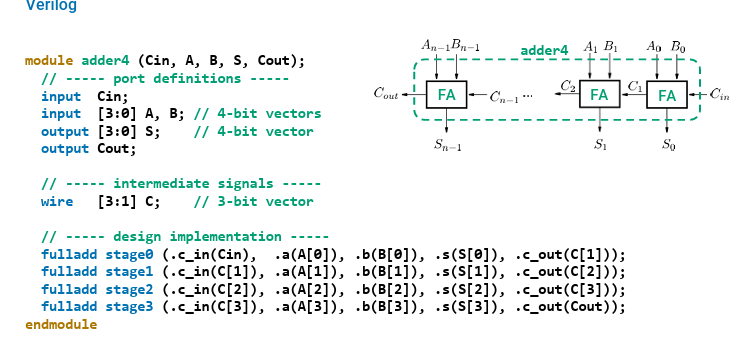
\includegraphics[scale=0.7]{72025-03-20.png}
            
        \end{center}
        
        
    \end{subparag} 
      \end{parag}
      
      
